\documentclass[twocolumn,10pt]{article}

\usepackage[english]{babel}
\usepackage[utf8]{inputenc}
\usepackage[T1]{fontenc}
\usepackage{listings}
\usepackage{graphicx}
\usepackage{comment}
\usepackage{amsmath}
\usepackage{hyperref}



\title{Assessed Coursework 2 Report\linebreak Distributed Algorithms and Systems}

\author{Willian de Oliveira Barreiros Junior\\
Matric Number: 2105514\\
 guns945@gmail.com\\}

\begin{document}
\maketitle

\section{Introduction}
This report regards the implementation details of a bidding system. The system consists of two java programs, a central server and a client. The system was conceived to ensure, first, data consistency, second, scalability, and finally, efficiency with multiple clients.

This report is divided into four parts, a thoroughly explanation on the server implementation and the structures used by it, the details on the client implementation, the tests performed, and finally, the conclusion, containing some final observations on the final implementation, the tests and possible future improvements.

The source code from this coursework can also be found at
\url{https://github.com/WillianJunior/DASProject1}

\section{Server Implementation}
The server was thought to be multithreaded, having one thread for each open auction. This way, the load on the server main thread will be reduced, this way, also reducing the delay between server-side operations. A diagram containing the main server operations can be seen in figure \ref{fig:diag}. Each operation will be described separately.

\begin{figure}[h]
\centering
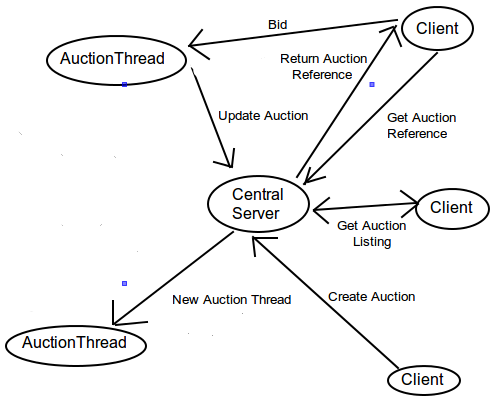
\includegraphics[scale=0.4]{diagram.png}
\caption{Main server operations}
\label{fig:diag}
\end{figure}

\subsection{Login/Logout}
Even that it is not shown in the diagram of figure \ref{fig:diag}, the login and logout are implicit operations. Both of them are handled by the server's main thread.

The user subsystem consists, in addition to the login and logout operations, of a list of users. This list keeps the user even if he/she is disconnected.

A short stub of the \textit{User} class can be seen at listing \ref{lstuser}. One important attribute to notice is the client callback reference. With this attribute the auction threads are able to notify the interested users about changes on the auction status (e.g. new bid, auction closed, etc).

\begin{lstlisting}[caption=\textit{User} class main methods and attributes, label=lstuser, language=java]
public class User 
  implements Serializable {
	
 private String name;
 private boolean connected;
 private RmiClientCallback client;

 public boolean isConnected ();
 public void connect 
   (RmiClientCallback client);				
 public void disconnect ();
 public RmiClientCallback getClient ();
}
\end{lstlisting}

One possible fault that could happen is: what if the client get disconnected without notifying the server? This would cause a RMI exception on the auction thread when notifying the user about some change on the auction status. This was treated in two different ways. First, the server main thread's constructor instantiate a \textit{Timer} object with a live clients checker. The \textit{Timer} will call a \textit{run} method on the live clients checker that will update the \textit{User}'s list on the server's main thread. Second, the auction thread is tolerant to the RMI exception thrown when the client is inaccessible. This way, the server is fault tolerant when regarding the client-side (e.g. the client crashes).

\subsection{Auction Creation}
As stated before, if the auction threads are separated from the main thread the influence that each auction have on the others performance is barely noticeable (unless we have a  ridiculously large number of auction threads). However, the server still needs to maintain a reference of all auctions for other operations (e.g. listing). Given that constraint, the auctions are stored in a \textit{volatile} structure, in a manner that every auction thread has access to its corresponding auction. 

The same structure that contains all auctions also have the reference for the thread that will handle its operations (if only the auction is still open, otherwise, the reference will be \textit{null}). The thread reference will be needed later.

There is an unresolved bug on the server's main thread regarding auction creation. It is possible that the creation of a new auction thread is unsuccessful, throwing an uncatched exception. More details about this bug and how it was found can be found in the test section of this report.

All concurrency problems related to the auction list will be addressed later on this section.

\subsection{Bidding}
One of the most important operations is (not surprisingly) bidding. From the server-side viewpoint the bidding is done by the corresponding auction thread. Given the implemented architecture, the bidding method implementation is trivial. The bidding consists on checking out if the bid is valid, updating the item value, and lastly, notifying the owner (if reachable).

As stated before, the intention was to maximize the concurrency level, and since the server's main thread guarantee that there will be only one thread per open auction, the access to a given auction don't need any locks or synchronisation. 

\subsection{Auction Listing}
The last of the main operations on the server-side is auction listing. There are two types of listing, the full list or the list of open auctions. This two operations would, on theory, have a trivial implementation, however, as it will be explained later, there was some racing conditions when the server load was too high. Not considering the racing conditions, the implementation of the listings is: extract all auctions from the server's auction list, and, if only the open auctions are needed, only copy the open ones.

\subsection{Racing Conditions, Concurrency and Some Semaphores}
The idea of a lock-free, concurrently accessed structure was too good to be true. As the server went through its first stress test, the first problem arose: a racing condition between the listing and writing methods on the auction list. It is expected that the listing method should have a write lock on the list, but only for new insertions, not for updates. Given that the only fields that are updatable on an auction are the current value of an item and its status (i.e. open/closed auction), and that they can't be updated in a single high-level operation, there should be no problem on listing and updating an auction item cost concurrently. When looking at the machine level,the update can be done in one CPU operation.

Unfortunately, java does not allow concurrent access for reading and writing on the same list structure, even if is impossible to reach an inconsistent state. 

Given the way java works with concurrency and also the racing condition between listing and adding a new auction to the list, we have some critical sections that need mutual exclusion. In order to solve this problem, first we need to define how many types of critical sections that need mutual exclusion. The answer is two, writers and readers. All listing operations can be said to be readers, and the bid and create a new auction operations are considered writers.

The mutual exclusion can be done easily by applying a lock on the critical section. Although it would work, this solution have one huge problem: it completely destroy all concurrency on the auction list, related to this four operations. The problem is that more that one writing operation can occur at the same time without provoking inconsistencies. The same goes for reading operations (for obvious reasons).

The mutual exclusion between readers and writers was implemented using semaphores, in a way that it is guaranteed, first of all, the mutual exclusion between readers and writers, second, the concurrency operation of multiple readers or multiple writers, and finally, there can be no starvation. To make easier to maintain and debug, a lock and unlock methods were implemented, as shown in listing \ref{lstsem}.

The needed variables for this mutual exclusion  algorithm is, a semaphore for the readers and one for the writers, and a simple lock. Assuming that A and B are the types of operations (i.e. reader or writer), and A is different that B, if we want to start a operation A, we call \textit{myLock(A, B)}, and at the end, \textit{myUnlock(A)}.

\begin{lstlisting}[caption=Semaphore operations, label=lstsem, language=java]
Semaphore reader = 
   new Semaphore(Integer.MAX_VALUE);
Semaphore writer = 
   new Semaphore(Integer.MAX_VALUE);
ReentrantLock multex = 
new ReentrantLock();

void myLock (Semaphore mySem, 
     Semaphore itsSem) {
   multex.lock();
   itsSem.acquireUninterruptibly
      (Integer.MAX_VALUE);
   itsSem.release(Integer.MAX_VALUE);
   mySem.acquireUninterruptibly();
   multex.unlock();
}

void myUnlock (Semaphore sem) {
   sem.release();
}
\end{lstlisting}

By surrounding the critical sections with this lock, and assuming that we want to execute an operation A, what happens is: 

\begin{lstlisting}
1. Check if there is an operation B 
  already executing, locking itself 
  if there is.
2. Decrement the semaphore A, meaning 
  that there is an operation A 
  in course.
3. After finishing the critical 
  section, Increment the semaphore A.
\end{lstlisting}

It is worth noticing that steps 1. and 2. are within a critical section themselves, thus, needing a lock.

In the worst case scenario, there would be a queue of alternating A and B operations. On this scenario the access to the auction list would be serially. The efficiency for this algorithm will be measured on the testing section.

\section{Client Implementation}
The implementation of the client is mostly IO and calls to the server. There are only a few point worth mentioning.

\subsection{Login/Logout}
In the same way that the client can be disconnected from the server without notifying it, causing problems (however, not on this implementation), the server can also drop the connection with the clients. If not treated, it would crash the client application.

However, this exception was also treated. Whenever the server drops the connection, the client application acknowledges it and keep trying to re-establish the connection with the server. The same thing happens if, at the start of the client execution, the server is offline.

\subsection{Bidding}
From the client's viewpoint it is a little bit trickier to perform a bid. The hole process is also visible at figure \ref{fig:diag}. 

First, the client needs to get the reference to the auction thread from the server's main thread. If the auction is not open the server will return a \textit{null} reference.

Finally, the client will perform the bid directly at the auction thread.

\subsection{Callbacks}
One parameter for the auction creation and bid server operations is the client's self reference. This way whenever there is any change that concerns this client, it will be notified.

\subsection{Some More Error Handling}
If the client loses the connection with the server while not doing anything it will only need to attempt the reconnection. However, if the connection drops in the middle of an operation (e.g. an auction creation) an exception will be thrown. The current implementation assures that the client is tolerant to this kind of failure, not crashing if this happens.

\section{Tests and Results Analysis}
To ensure fully functionality of the auctions system and to measure its efficiency some tests were performed.

\subsection{Stress Test}
The first step is to assure that the system is fault-proof, and can support a great load without crashing. In order to ensure it a new client class was created only for test purposes, the \textit{ElatedClient}. This class will basically repeatedly run, either the same operation or a random operation, with a configurable delay between each call.

The stress test consist on starting a server and run one \textit{ElatedClient} of each type with no delay whatsoever.

The first time this test ran it almost immediately crashed the server. The first bug found was the racing condition between readers and writers, mentioned before.

The second try the server held a little bit longer, but still crashed. This time due to a documented bug regarding the serialisation/deserialisation of the \textit{Calendar} object, which was used to represent the end and removal date/time of each auction. The fix was simple, change the \textit{Calendar} object to a \textit{long} field with the milliseconds value of the chosen date/time. This bug was actually a good thing. Later testing showed that the transaction time reduced radically after making the change. This is due to the high cost of serialising and deserialising an object.

At the third time the server held and did not crashed, even after a few minutes.

All the aforementioned tests were performed on the authors laptop.

\subsection{System Efficiency}
The final tests are related on how does the server handle different types of load. The efficiency tests consist on:

\begin{lstlisting}
1. Test insertion only
2. Test bidding only
3. Test listing all auctions only
4. Test listing open auctions only
5. Test an estimated mixed load
\end{lstlisting}

All tests were performed on the authors laptop and also on multiple physical machines located on the level 3 computer lab of the Boyd Orr Building. The first four tests were performed with different numbers of clients (1-5 clients). All tests were performed with no delay between operations.

As we can see in both test configurations, the bidding has the lowest time cost, which is expected since that is, probably, the mostly used operation, and definitely the operation that most needs a low execution time.

The test represented by table 2 was done with all clients running concurrently. The interesting feature at this table is that, even with a mixed load, which was expected to degrade the performance of the read/write operations (discussed on subsection 2.5), the time taken to perform bidding operations is still excellent in comparison with the results of table 1.

When testing the server on the lab, trying to test the auction creation, after few seconds the sever crashed due to low memory. This happened because the server couldn't instantiate any more threads. Although this fault should be treated, it is odd that it only happened on the lab computers, which makes me believe that the problem might be due to some JVM configuration (memory or max number of threads limit).

Yet, the most interesting results are the ones on table 3. The tests using multiple physical machines showed that the server can still hold more than six clients without any problem.

\begin{table}
\label{tbltpo}
\begin{center}
\begin{tabular}{ | l | c | c | c | c | c |}
\hline
No of Clients & 1 & 2 & 3 & 4 & 5 \\
\hline
Auction Creation & 3.44 & 2.44 & 3.80 & 4.53 & 6.14 \\
Bidding & 2.11 & 2.10 & 2.51 & 3.05 & 4.01 \\
Listing All & 10.23 & 8.00 & 12.87 & 18.74 & 64.76 \\
Listing Open & 12.73 & 9.96 & 13.02 & 20.85 & 53.35 \\
\hline
mean & 7.13 & 5.62 & 8.05 & 11.79 & 32.06 \\
\hline  
\end{tabular}
\end{center}
\caption{Time needed for each operation on the laptop with only one physical machine (time in milliseconds)}
\end{table}

\begin{table}
\label{tbltpm}
\begin{center}
\begin{tabular}{ | l | c | }
\hline
Auction Creation & 3.44 \\
\hline
Bidding 1 & 2.11\\
\hline
Bidding 2 & 2.11\\
\hline
Listing All & 10.23\\
\hline
Listing Open & 12.73 \\
\hline
\end{tabular}
\end{center}
\caption{Time needed for each operation on the laptop with only one physical machine with a mixed load (time in milliseconds)}
\end{table}

\begin{table}
\label{tblab}
\begin{center}
\begin{tabular}{ | l | c | c | c | c | c | c |}
\hline
No of Clients & 1 & 2 & 3 & 4 & 5 & 6 \\
\hline
Auction Creation & 2.77 & 3.22 & 3.61 & 3.48 & 3.55 & 3.53 \\
Bidding & 0.46 & 0.43 & 0.44 & 0.44 & 0.44 & 0.43 \\
Listing All & 2.14 & 1.65 & 1.79 & 1.90 & 1.71 & 1.71 \\
Listing Open & 1.82 & 2.00 & 2.03 & 2.11 & 2.11 & 1.98 \\
\hline
mean & 1.80 & 1.83 & 1.97 & 1.98 & 1.95 & 1.91 \\
\hline  
\end{tabular}
\end{center}
\caption{Time needed for each operation on the lab with one physical machine per client (time in milliseconds)}
\end{table}

\section{Final Remarks}
After analysing the tests results we can conclude that the auction system was successfully implemented, guaranteeing all the expected features mentioned at the introduction.

Even so, there are still some improvement that can be done. 

First, and most importantly, the out of memory fault should be treated properly.

Some optimisations can also be done. One example is to break the auction list into two, one of open auctions and other of closed ones.

There is also the possibility of race condition on the users list on the server's main thread. This possibility wasn't fully investigated.

Finally, since this is a distributed systems course, a distributed server would be a great addition. Given the current architecture, the evolution of the system to a distributed server system wouldn't take much impact on the client-side implementation. If this was to be implemented, it would probably be a ring of equal servers with static load balance (only at auction allocation time) and at most a lightweight master server to give the clients access to the servers ring.

\end{document}